\subsection*{Las 7 emociones básicas}
Las emociones evolucionaron para cumplir la función de promover la supervivencia física, pero el desarrollo de la cultura humana también ha impulsado la evolución de las emociones en el sentido de que esta
s cumplan funciones relativas a metas sociales, tales como llevarse bien con los demás y avanzar en la comunidad. Las emociones básicas tienen funciones sociales además de las de supervivencia \cite{rulicki2012cnv}.

Estas siete emociones básicas son:
\begin{itemize}
\item \textbf{Alegría:} Sensación dichosa de placer y bienestar \cite{rulicki2012cnv}.
\item \textbf{Tristeza:} Sensación opresiva de pérdida o carencia que produce desánimo \cite{rulicki2012cnv}.
\item \textbf{Miedo:} Sensación de agitación causada por una percepción de peligro debida a riesgos físicos, morales, o la presencia de dolor \cite{rulicki2012cnv}.
\item \textbf{Enojo:} Sensación perturbadora que resulta de una ofensa, una torpeza propia o un obstáculo natural. Generalmente incluye el deseo de reaccionar agresivamente \cite{rulicki2012cnv}.
\item \textbf{Asco:} Sensación de repugnancia debida a la percepción de un estímulo desagradable a los sentidos \cite{rulicki2012cnv}.
\item \textbf{Desprecio:} Sensación de rechazo o desestimación hacia otra persona o cosa, por considerarla inferior, indigna o carente de valor \cite{rulicki2012cnv}.
\item \textbf{Sorpresa:} Sensación súbita e inesperada de asombro \cite{rulicki2012cnv}.
\end{itemize}

\begin{figure}[h]
    \centering
    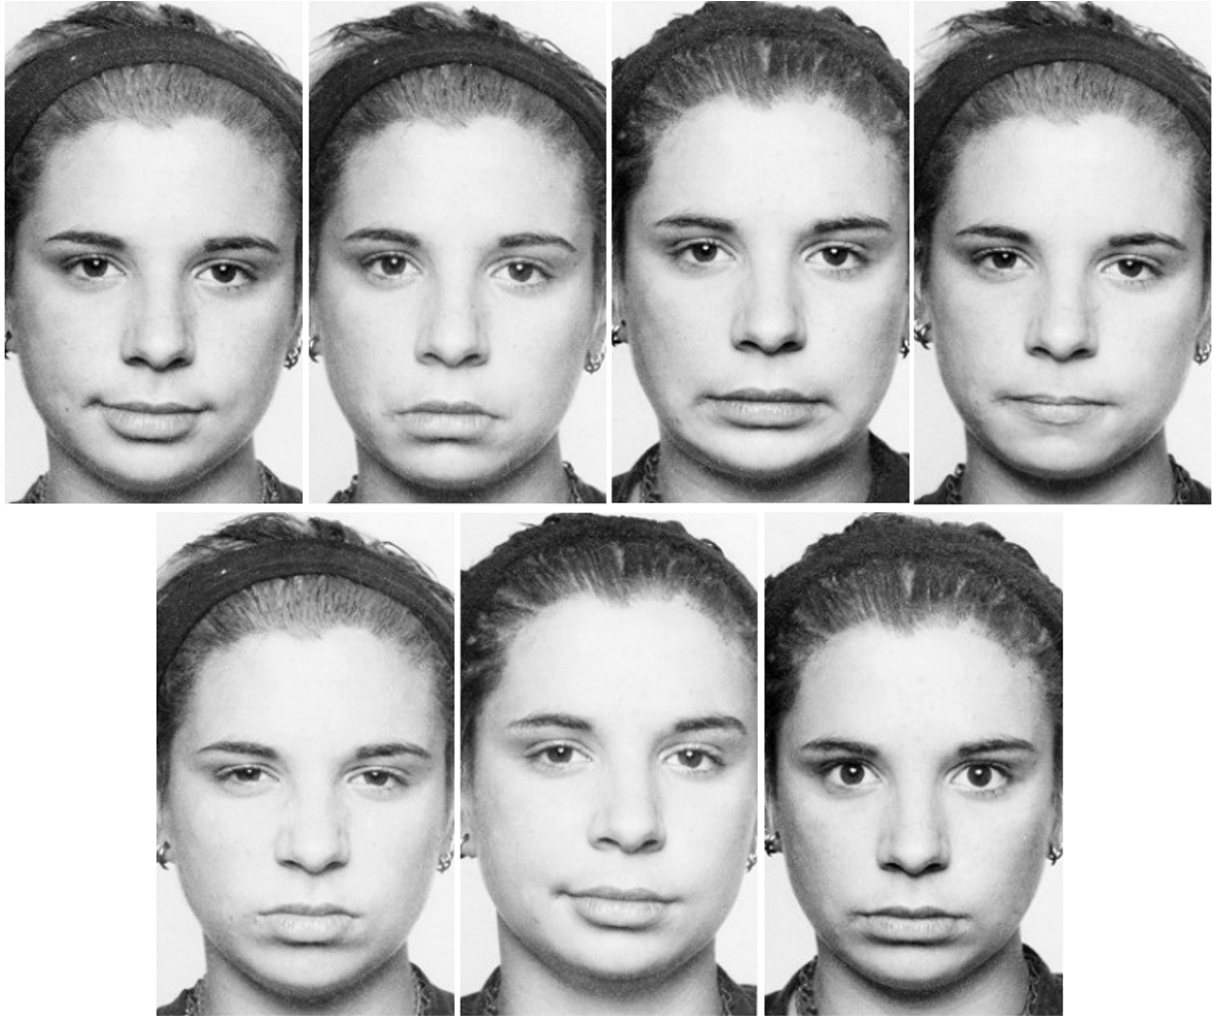
\includegraphics[width=0.6\textwidth]{Emociones.png}
    \caption{Gestos de distintas emociones \cite{ekman2017rostro}.}
    \label{fig:Emociones}
\end{figure}

\subsubsection*{Las señales faciales de las emociones}
Las señales faciales son las configuraciones de los distintos rasgos particulares de cada emoción, que son producidas por movimientos involuntarios en los músculos del rostro. Según Ekman, las expresiones de las emociones nos dan información acerca de lo que está ocurriendo dentro de la persona, lo que posiblemente ocurrió antes de que se desarrollara la emoción y aquello que puede llegar a pasar en consecuencia de la emoción. Para esto se utiliza el sistema FACS (Facial Action Coding System), que es un sistema de codificación que recoge todos movimientos expresivos del rostro en unidades de acción (AU) \cite{ekman2017rostro}.

\begin{table}[H]
\centering
\begin{tabular}{|c|c|}
\hline
\textbf{AU} & \textbf{Acción} \\ \hline
1             & Levantamiento interior de ceja      \\ \hline
2             & Levantamiento exterior de ceja      \\ \hline
4             & Bajar cejas                         \\ \hline
5             & Levantamiento del párpado superior  \\ \hline
6             & Levantamiento de mejillas           \\ \hline
7             & Apretar párpados                    \\ \hline
8             & Labios encimados uno de otro        \\ \hline
9             & Arrugar nariz                       \\ \hline
10            & Levantamiento del labio superior    \\ \hline
11            & Profundidad nasolabial              \\ \hline
12            & Tiramiento labial esquinal          \\ \hline
13            & Tiramiento labial frontal           \\ \hline
14            & Hoyuelo facial                      \\ \hline
15            & Depresión labial esquinal           \\ \hline
16            & Depresión labial frontal            \\ \hline
17            & Levantamiento de barbilla           \\ \hline
18            & Arruga labial                       \\ \hline
19            & Muestro de lengua                   \\ \hline
20            & Apretar los labios                  \\ \hline
21            & Apretamiento de cuello              \\ \hline
22            & Embudo labial                       \\ \hline
23            & Morder labios                       \\ \hline
24            & Presión labial                      \\ \hline
25            & Deslizamiento labial                \\ \hline
26            & Caída de la mandíbula               \\ \hline
27            & Apretamiento bucal                  \\ \hline
28            & Lamido labial                       \\ \hline
29            & Tracción de la mandíbula            \\ \hline
\end{tabular}
\caption{Lista de Unidades de acción y descripciones de acción.}
    \label{cuadro:AU}
\end{table}

\begin{table}[H]
\centering
\begin{tabular}{|c|c|}
\hline
\textbf{AU} & \textbf{Acción} \\ \hline
30            & Deslizamiento de mandíbula          \\ \hline
31            & Contracción mandibular              \\ \hline
32            & Mordida labial                      \\ \hline
33            & Succión de mejillas                 \\ \hline
34            & Inflar mejillas                     \\ \hline
35            & soplido de mejillas                 \\ \hline
36            & Protuberancia de lengua             \\ \hline
37            & Limpieza labial                     \\ \hline
38            & Dilatado nasal                      \\ \hline
39            & Compresión nasal                    \\ \hline
\end{tabular}
\caption{Lista de Unidades de acción y descripciones de acción.(continuación)}
    \label{cuadro:AU}
\end{table}

\subsection*{Como reconocer las emociones en los demás}

\subsubsection*{Alegría}
El truco para reconocer correctamente la alegría está en los ojos. Concretamente, en las temidas patas de gallo. Si no aparecen estas características arrugas en el contorno exterior de los ojos, la sonrisa no se considera espontánea, sino una sonrisa social o intencionada. Los dos movimientos musculares o unidades de acción más características de la alegría son la elevación simétrica de las comisuras de los labios (AU12) y el ascenso de las mejillas (AU6) \cite{ReconocerLasEmociones}.

\begin{figure}[h]
    \centering
    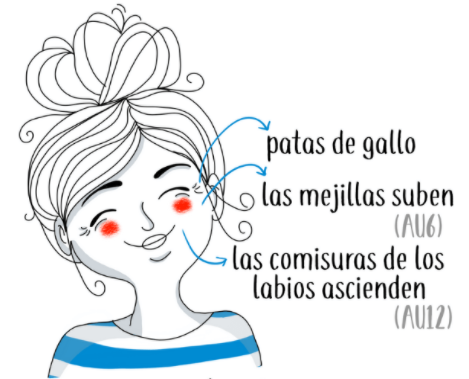
\includegraphics[width=0.25\textwidth]{Alegria.png}
    \caption{Rasgos de alegría \cite{ReconocerLasEmociones}.}
    \label{fig:Alegria}
\end{figure}

\subsubsection*{Sorpresa}
Las tres unidades de acción más características de la sorpresa son la elevación simétrica de las cejas hacia el exterior (AU2), la apertura desorbitada de los párpados (AU5) y la caída de la mandíbula (AU26). El truco para reconocer correctamente la sorpresa está en los ojos y en la mandíbula. Los ojos parecen desorbitar, por efecto de la subida de los párpados superiores. Y lo que es más curioso, queda al descubierto la parte blanca de la esclerótica por encima del iris, que normalmente no vemos \cite{ReconocerLasEmociones}.

\begin{figure}[h]
    \centering
    \includegraphics[width=0.25\textwidth]{sorpresa.png}
    \caption{Rasgos de sorpresa \cite{ReconocerLasEmociones}.}
    \label{fig:Sorpresa}
\end{figure}

\subsubsection*{Tristeza}
Las unidades de acción más características de la tristeza son la elevación de las cejas hacia el interior (AU1), la caída de las comisuras de los labios (AU15), y la subida del mentón (AU17). El truco para reconocer correctamente la tristeza está en el comportamiento de las cejas. Lo más habitual es que, al subir hacia el interior, la activación del músculo frontal forme unas arrugas horizontales en el centro de la frente \cite{ReconocerLasEmociones}.

\begin{figure}[h]
    \centering
    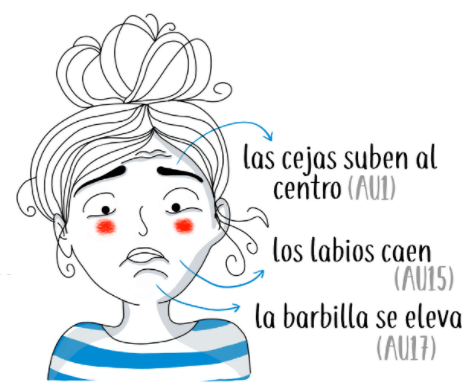
\includegraphics[width=0.25\textwidth]{Tristeza.png}
    \caption{Rasgos de tristeza \cite{ReconocerLasEmociones}.}
    \label{fig:Tristeza}
\end{figure}

\subsubsection*{Miedo}
El truco para reconocer correctamente el miedo está en fijarnos bien en los ojos, y no confundirlos con los de la sorpresa. Las dos unidades de acción más características del miedo son la elevación de los párpados superiores (AU5), y la retracción o estiramiento horizontal de los labios (AU20) \cite{ReconocerLasEmociones}.

\begin{figure}[h]
    \centering
    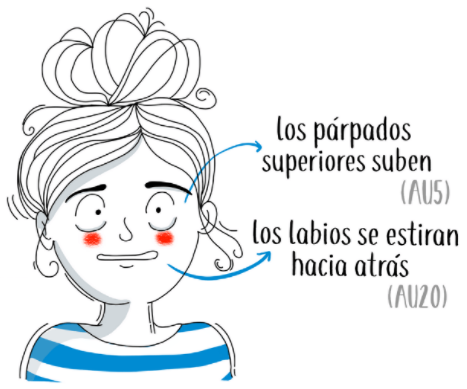
\includegraphics[width=0.25\textwidth]{Miedo.png}
    \caption{Rasgos de Miedo \cite{ReconocerLasEmociones}.}
    \label{fig:Miedo}
\end{figure}

\subsubsection*{Ira}
Las tres unidades de acción más características de la ira son juntar y bajar las cejas sobre la nariz (AU4), la tensión en los párpados inferiores (AU7) y la proyección de la mandíbula hacia adelante (AU29). El truco para reconocer correctamente la ira está en el ceño fruncido, formado por las típicas arrugas sobre la nariz al juntar y bajar las cejas \cite{ReconocerLasEmociones}.

\begin{figure}[h]
    \centering
    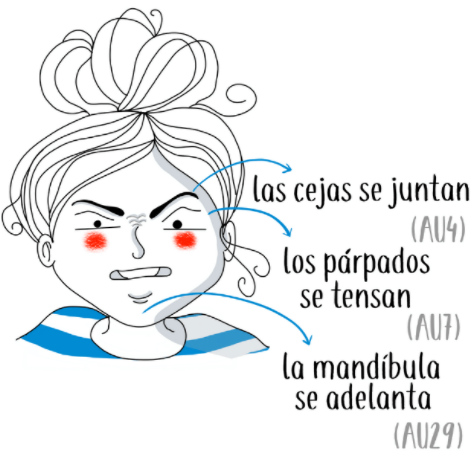
\includegraphics[width=0.25\textwidth]{Ira.png}
    \caption{Rasgos de ira \cite{ReconocerLasEmociones}.}
    \label{fig:Ira}
\end{figure}

\subsubsection*{Asco}
Las dos unidades de acción más características del asco son arrugar la nariz (AU9), y elevar el labio superior (AU10). El truco para reconocer correctamente el asco está en la activación del pliegue nasolabial, fácilmente reconocible porque el labio superior asciende y la nariz se arruga \cite{ReconocerLasEmociones}.

\begin{figure}[h]
    \centering
    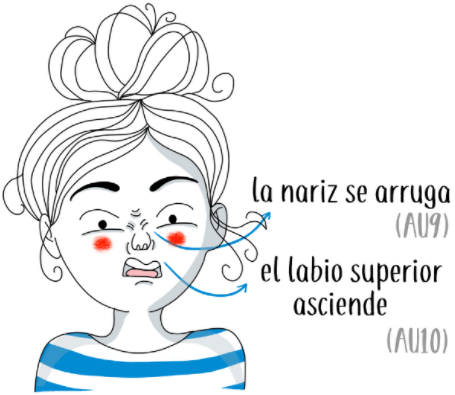
\includegraphics[width=0.25\textwidth]{Asco.png}
    \caption{Rasgos de asco \cite{ReconocerLasEmociones}.}
    \label{fig:Asco}
\end{figure}

\subsubsection*{Desprecio}
La única unidad de acción características del desprecio es la retracción de una de las comisuras de los labios hacia la mejilla (AU14), formando el típico hoyuelo en un solo lado de la cara, o acentuando su existencia.El truco para reconocer correctamente el desprecio está en el típico hoyuelo, formado en una sola de las mejillas cuando los labios se retraen hacia un lado de la cara. El problema está en que no siempre se aprecia con claridad, sobre todo si la microexpresión es leve y rápida \cite{ReconocerLasEmociones}.

\begin{figure}[h]
    \centering
    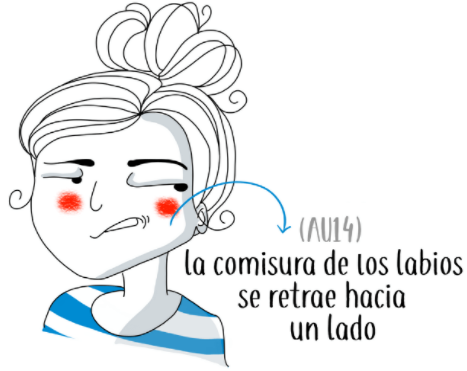
\includegraphics[width=0.25\textwidth]{Desprecio.png}
    \caption{Rasgos de desprecio \cite{ReconocerLasEmociones}.}
    \label{fig:Desprecio}
\end{figure}

\subsection*{Visión por computadora}
\subsubsection*{OpenCV}
OpenCV es una biblioteca de software de visión por computadora y de aprendizaje automático (\textit{Machine learning}) de código abierto. OpenCv se creó para aplicaciones de visión por computadora y para acelerar el uso de la percepción de la máquina en productos comerciales. Al ser un producto con licencia BSD, facilita que las empresas utilicen y modifiquen el código. La biblioteca tiene más de 2500 algoritmos optimizados que incluyen un conjunto completo de algoritmos de aprendizaje automático y visión por computadora clásicos y de última generación. Estos algoritmos se pueden utilizar para detectar y reconocer rostros, identificar objetos, clasificar acciones humanas en videos, entre otros. OpenCV tiene más de 47 mil usuarios en la comunidad y un número estimado de descargas superior a 18 millones. La biblioteca se utiliza ampliamente en empresas, grupos de investigación y organismos gubernamentales. Tiene interfaces C ++, Python, Java y MATLAB y es compatible con Windows, Linux, Android y Mac OS \cite{OpenCV}.

\subsubsection*{SimpleCV}
SimpleCV es un marco de código abierto para crear aplicaciones de visión por computadora. Con él, obtiene acceso a varias bibliotecas de visión por computadora de alta potencia, como OpenCV, sin tener que aprender primero sobre profundidades de bits, formatos de archivo, espacios de color, administración de búfer, valores propios o almacenamiento de matriz versus mapa de bits. Esta es la visión por computadora simplificada \cite{SimpleCV}.

\subsubsection*{Accord.NET Framework}
Accord.NET Framework es un marco de aprendizaje automático .NET combinado con bibliotecas de procesamiento de audio e imagen completamente escritas en C\#. Es un marco completo para crear aplicaciones de visión por computadora, audición por computadora, procesamiento de señales y estadísticas, incluso para uso comercial. Un conjunto completo de aplicaciones que proporciona un comienzo rápido para comenzar a funcionar rápidamente, y una extensa documentación y wiki ayudan a completar los detalles \cite{Accord.NET}.

\subsubsection*{BoofCV}
BoofCV es una biblioteca de código abierto escrita desde cero para la visión por computadora en tiempo real. Su funcionalidad cubre una variedad de temas, procesamiento de imágenes de bajo nivel, calibración de la cámara, detección / seguimiento de funciones, estructura desde el movimiento, detección fiducial y reconocimiento. BoofCV ha sido lanzado bajo una licencia Apache 2.0 para uso académico y comercial \cite{BoofCV}.

\subsection*{Aprendizaje automático}
\subsubsection*{Keras}
Keras es una API de aprendizaje profundo escrita en Python, que se ejecuta sobre la plataforma de aprendizaje automático TensorFlow. Fue desarrollado con un enfoque en permitir una experimentación rápida. Ser capaz de pasar de la idea al resultado lo más rápido posible es clave para hacer una buena investigación. Ofrece APIs consistentes y simples, minimiza la cantidad de acciones del usuario necesarias para casos de uso comunes y proporciona mensajes de error claros y procesables. También cuenta con una extensa documentación y guías para desarrolladores \cite{Keras}.

\subsubsection*{TensorFlow}
TensorFlow es una plataforma de código abierto de extremo a extremo para el aprendizaje automático. Cuenta con un ecosistema integral y flexible de herramientas, bibliotecas y recursos de la comunidad que les permite a los investigadores innovar con el aprendizaje automático y, a los desarrolladores, compilar e implementar con facilidad aplicaciones con tecnología de AA. TensorFlow ofrece varios niveles de abstracción para que puedas elegir el que se adecue a tus necesidades. Compila y entrena modelos mediante la API de alto nivel de Keras, que ayuda a que los primeros pasos con TensorFlow y el aprendizaje automático sean sencillos \cite{TensorFlow}.

\subsubsection*{PyTorch}
Es un paquete de Python diseñado para realizar cálculos numéricos haciendo uso de la programación de tensores. Además permite su ejecución en GPU para acelerar los cálculos. Normalmente PyTorch es usado tanto para sustituir numpy y procesar los cálculos en GPU como para la investigación y desarrollo en el campo del machine learning, centrado principalmente en el desarrollo de redes neuronales. PyTorch es una librería muy reciente y pese a ello dispone de una gran cantidad de manuales y tutoriales donde encontrar ejemplos. Además de una comunidad que crece a pasos agigantados. PyTorch dispone una interfaz muy sencilla para la creación de redes neuronales pese a trabajar de forma directa con tensores sin la necesidad de una librería a un nivel superior como pueda ser Keras para Theano o Tensorflow \cite{PyTorch}.